\chapter{Perancangan ABS MVC Framework}

Bab ini membahas tentang rancangan ABS MVC Framework yang penulis buat sebelum melakukan tahap implementasi kode.

\section{Gambaran Umum}

ABS MVC Framework merupakan sebuah alat bantu yang dapat digunakan oleh para pengembang perangkat lunak dalam membuat sebuah aplikasi berbasis web dengan menggunakan bahasa pemodelan ABS. Layaknya MVC Framework yang lain seperti Play Framework (JAVA) \footnote{https://www.playframework.com/}, Laravel (PHP) \footnote{http://laravel.com/} dan Code Igniter (PHP) \footnote{https://github.com/bcit-ci/CodeIgniter}, ABS MVC Framework dibuat dengan tujuan untuk membantu para pengembang perangkat lunak dalam menerapkan pola Model-View-Controller (MVC) untuk keperluan pengembangan aplikasi web. Oleh karena itu, terdapat beberapa fitur utama yang harus dimiliki oleh ABS MVC Framework sebagai sebuah MVC Framewrok yang diantara adalah:

\begin{enumerate}
    \item ABS MVC Framework harus dapat membantu pengguna \textit{framework} untuk dapat menghasilkan sebuah halaman web yang statis maupun dinamis.
    \item ABS MVC Framework harus dapat membantu pengguna \textit{framework} untuk dapat memisahkan kode yang mereka buat kedalam komponen Model, View dan Controller.
    \item Setiap komponen MVC yang dibuat harus memiliki karakteristik yang jelas sehingga dapat dibedakan mana komponen Model, View dan Controller.
    \item ABS MVC Framework harus dapat membantu pengguna \textit{framework} dalam memetakan setiap HTTP \textit{request} yang diterima kedalam setiap operasi yang spesifik sehingga diperoleh sebuah halaman web yang sesuai.
    \item ABS MVC Framework harus dapat memebantu pengguna \textit{framework} dalam menerima dan memproses \textit{input} yang diberikan oleh pengguna aplikasi web dalam bentuk HTTP POST atau GET data. 
\end{enumerate}

Berdasarkan rincian fitur di atas, penulis membuat sebuah rancangan untuk ABS MVC Framework yang nantinya akan dijadikan acuan dalam proses implementasi.

\section{Rancangan ABS MVC Framework}

Setelah adanya pemaparan tentang gambaran umum fitur yang harus dimiliki oleh ABS MVC Framework, penulis membuat sebuah desain tentang bagaimana alur kerja ABS MVC Framework dimuali dari mendapatkan HTTP \textit{request} sampai dengan menampilkan halaman web pada \textit{web browser}. Berikut ini adalah desain yang penulis buat untuk ABS MVC Framework:

\begin{figure}
    \centering
    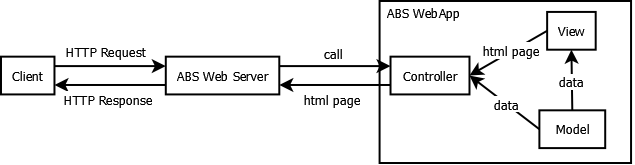
\includegraphics[width=0.8\textwidth]{img/abs-mvc.png}
    \caption{Rancangan ABS MVC Framework}
    \label{fig:mvcFrameworkDesign}
\end{figure}

Seperti yang terlihat pada gambar \ref{fig:mvcFrameworkDesign} di atas, alur pembuatan halaman web dimulai dari sebuah HTTP \textit{request} yang dikirimkan oleh pengguna web kepada \textit{web server} melalui aplikasi \textit{web browser} yang mereka gunakan. Setelah HTTP \textit{request} tersebut diterima oleh \textit{web server}, berikutnya adalah meneruskan \textit{request} tersebut kapada ABS MVC Framework untuk memperoleh halaman web yang diinginkan. Setelah \textit{web server} berhasil memperoleh halaman web yang diinginkan, selanjutnya \textit{web server} akan memberikan halaman tersebut kepada \textit{web browser} untuk kemudian ditampilkan kepada pengguna web. Melalui mekanisme inilah seorang pengguna web dapat mengakses halaman web yang telah dibuat.\\

Berdasarkan pada rancangan tersebut, penulis menyimpulkan bahwa terdapat tiga buah isu yang harus diperhatikan dalam menyusun ABS MVC Framework yang diantaranya adalah:

\begin{enumerate}
    \item Bagaimana mekanisme pemetaan yang dapat dilakukan dalam memetakan setiap HTTP \textit{request} kedalam setiap komponen Controller pada ABS MVC Framework.
    \item Bagaimana mekanisme yang dapat dilakukan agar ABS MVC Framework dapat menerima dan memproses setiap HTTP POST dan GET data yang diterima oleh \textit{web server}.
    \item Bagaimana karakteristik setiap komponen MVC yang ada di pada ABS MVC Framework.
\end{enumerate}
\subsection{Mekanisme Pemetaan HTTP Request}

Dalam konteks pengembangan aplikasi web dengan menggunakan MVC Framework, setiap \textit{request} yang diberikan oleh pengguna aplikasi harus dipetakan kedalam setiap komponen Controller yang dibuat. Tujuannya adalah agar \textit{web server} dapat mengetahui dengan pasti komponen Controller manakah yang harus dipanggil pada saat menerima \textit{request} dari \textit{web browser}. Untuk dapat merealisasikan hal tersebut, dibutuhkan adanya mekanisme khusus yang dapat digunakan oleh pengguna \textit{framework} untuk dapat memetakan setiap \textit{request} yang diterima secara cepat dan mudah.

\begin{figure}
    \centering
    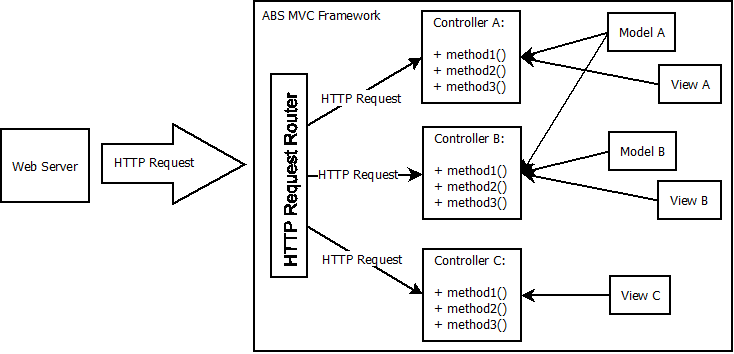
\includegraphics[width=0.8\textwidth]{img/mvc-routing-mechanism}
    \caption{Rancangan mekanisme pemetaan \textit{request} pada ABS MVC Framework}
    \label{fig:mvcRoutingMechanism}
\end{figure}

Seperti yang terlihat pada gambar \ref{fig:mvcFrameworkDesign} di atas, pada ABS MVC Framework proses pemetaan HTTP \textit{request} dilakukan oleh sebuah komponen yang bernama HTTP Request Router. Melalui komponen ini, setiap \textit{request} yang diberikan oleh \textit{web server} akan dipetakan kedalam setiap komponen Controller yang berada di dalam \textit{framework}. Dengan demikian, ABS MVC Framework akan dapat menghasilkan halaman web yang sesuai dengan permintaan dari \textit{web browser}.

\subsection{Mekanisme Penanganan HTTP POST dan GET data}

Seperti yang sudah penulis sebutkan pada rincian fitur ABS MVC Framework, salah satu fitur yang harus dimiliki oleh \textit{framework} ini selain dapat melakukan pemetaan HTTP Request kedalam komponen Controller adalah kemampuannya dalam menerima dan memperoses \textit{input} yang diberikan dalam bentuk HTTP POST dan GET data. Tujuan dari adanya fitur ini adalah agar aplikasi web yang dibuat dapat menerima \textit{input} dari pengguna dan menghasilkan sebuah halaman web yang dinamis. Untuk dapat merealisasikan hal tersebut, dibutuhkan adanya sebuah mekanisme yang dapat digunakan oleh \textit{web server} untuk dapat meneruskan HTTP POST dan GET data yang diterima dari \textit{web server} kepada ABS MVC Framework. Berikut ini adalah rancangan yang penulis buat untuk mengani HTTP POST dan GET data pada ABS MVC Framework.

\begin{figure}
    \centering
    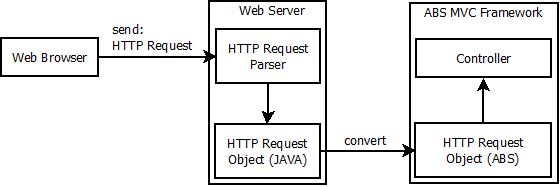
\includegraphics[width=0.8\textwidth]{img/mvc-http-input.png}
    \caption{Rancangan mekanisme penanganan \textit{input} pada ABS MVC Framework}
    \label{fig:mvcHttpInputMechanism}
\end{figure}

Terlihat pada gambar \ref{fig:mvcHttpInputMechanism} di atas, setiap HTTP \textit{request} yang diterima oleh \textit{web server} akan dibuat menjadi sebuah objek JAVA. Objek yang berisikan HTTP POST atau GET data ini nantinya akan dikonversi menjadi sebuah Objek ABS dan diberikan kepada ABS MVC Framework untuk kemudian digunakan oleh komponen Controller. Dengan menggunakan cara ini, pengguna ABS MVC Framework dapat menerima dan memproses \textit{input} yang diberikan oleh \textit{web server} melalui komponen Controller yang dibuat.

\subsection{Karakteristik komponen MVC pada ABS MVC Framework}

Salah satu tujuan dari penggunaan MVC Framework dalam proses pengembangan perangkat lunak adalah untuk membantu para pengembang dalam memecah kode program yang dibuat kedalam komponen Model, View dan Controller. Untuk dapat memecah kode program kedalam tiga buah komponen tersebut, perlu adanya karakteristik yang jelas yang dapat membedakan ketiga buah komponen tersebut. Oleh karena itu, penulis pelu mendefinisikan karakteristik dari setiap komponen MVC yang ada di dalam ABS MVC Framework untuk mempermudah para pengembang dalam mengelompokan kode program yang mereka buat.

Berikut ini adalah karakteristik yang sudah penulis rancang untuk setiap komponen MVC pada ABS MVC Framework:

\begin{itemize}
    \item \textbf{Model}: Komponen ini merupakan komponen yang merepresentasikan data pada aplikasi yang dibuat. Dalam membuat komponen Model ini, diharapkan komponen ini dibentuk sesederhana mungkin dengan hanya berisikan atribut-atribut yang berkaitan dengan data beserta \textit{method} aksesor dan mutatornya.Setiap kode yang mengandung proses bisnis aplikasi tidak boleh diletakan di dalam komponen ini.
    \item \textbf{View}: Komponen ini berperan dalam mempresentasikan data yang berasa dari komponen Model kepada pengguna aplikasi dalam bentuk halaman web. Dalam konteks pengembangan aplikasi web, diharapkan komponen ini dapat didefinisikan dengan menggunakan sintaks HTML untuk memudahkan para pengembang dalam proses pembuatannya. Selain itu, dikarenakan komponen ini ditujukan untuk menampilkan komponen Model yang diberikan, maka komponen ini harus bisa mengakses komponen Model secara langsung.
    \item \textbf{Controller}: Komponen ini merupakan komponen yang berisikan proses bisnis dari aplikasi web yang dibuat. Pada komponen inilah pengembang perangkat lunak akan memproses setiap \textit{input} yang diberikan oleh pengguna aplikasi dan mengintegrasikannya dengan komponen Model dan View dalam menghasilkan sebuah halaman web yang utuh. Komponen ini merupakan komponen utama dalam sebuah aplikasi web berbasis MVC dan oleh karenanya, keberadaan komponen ini tidak dapat dihilangkan dari dalam aplikasi web yang dibuat.
\end{itemize}

Sampai pada tahap ini, penulis telah berhasil membuat rancangan untuk ABS MVC Framework. Langkah berikutnya adalah melakukan proses implementasi (\textit{coding}) untuk dapat merealisasikan rancangan yan dibuat.
